\chapter{\ifenglish Background Knowledge and Theory\else ทฤษฎีที่เกี่ยวข้อง\fi}

การทำโครงงาน เริ่มต้นด้วยการศึกษาค้นคว้า ทฤษฎีที่เกี่ยวข้อง หรือ งานวิจัย/โครงงาน ที่เคยมีผู้นำเสนอไว้แล้ว ซึ่งเนื้อหาในบทนี้ก็จะเกี่ยวกับการอธิบายถึงสิ่งที่เกี่ยวข้องกับโครงงาน เพื่อให้ผู้อ่านเข้าใจเนื้อหาในบทถัดๆ ไปได้ง่ายขึ้น

\section{Fraction models}
ลักษณะของเศษส่วนที่ใช้สื่อความหมายมีหลายแบบ เช่น โดยแต่ละแบบมีจุดเด่นที่แตกต่างกันไป

\subsection{Area model}
Area model เป็นการใช้รูปทรงเรขาคณิตต่างๆ เช่น วงกลม สี่เหลี่ยม หรือรูปสามเหลี่ยม มาแบ่งส่วนเพื่อแสดงความหมายของเศษส่วน
\begin{figure}[h!tbp]
\begin{centering}
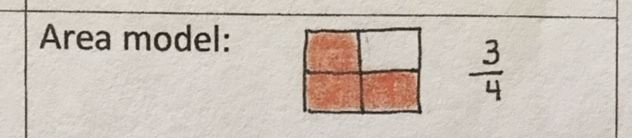
\includegraphics{Area_model.png}
\end{centering}
\caption[Area model]{Area model of fraction 3/4}
\end{figure}

\subsection{Set model}
Set model เป็นการใช้กลุ่มของวัตถุที่เหมือนกันมาแบ่งกลุ่มเพื่อแสดงความหมายของเศษส่วน เช่น การใช้ลูกปัดสีแดงและสีขาวมาแบ่งกลุ่มเพื่อแสดงเศษส่วน
\begin{figure}[h!tbp]
\begin{center}
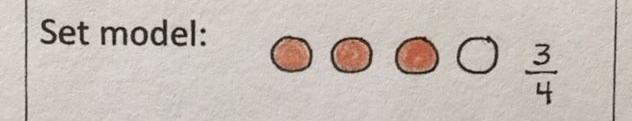
\includegraphics{Set_model.png}
\end{center}
\caption[Set model]{Set model of fraction 3/4}
\end{figure}

\subsection{Length model}
Length model เป็นการใช้เส้นตรงเพื่อแสดงความหมายของเศษส่วน โดยจะเป็นการใช้เส้นตรงยาว 1 หน่วยมาแบ่งเป็นส่วนๆ
\begin{figure}[h!tbp]
\begin{center}
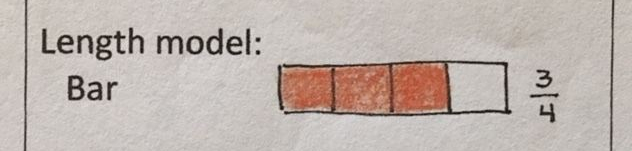
\includegraphics{Length_model.png}
\end{center}
\caption[Length model]{Length model of fraction 3/4}
\end{figure}


% This code demonstrates how to get a landscape table or figure. It
% uses the package lscape to turn everything but the page number into
% landscape orientation. Everything should be included within an
% \afterpage{ .... } to avoid causing a page break too early.


\section{\ifenglish%
\ifcpe CPE \else ISNE \fi knowledge used, applied, or integrated in this project
\else%
ความรู้ตามหลักสูตรซึ่งถูกนำมาใช้หรือบูรณาการในโครงงาน
\fi
}

ความรู้จากหลักสูตรวิชา object oriented programming ในด้านการใช้ Figma ในการออกแบบ UI ของแอปพลิเคชัน
ความรู้จากหลักสูตรวิชา intro hci ซึ่งเป็นวิชาที่เกี่ยวข้องกับการออกแบบและพัฒนา UX/UI โดยเน้นการสร้างประสบการณ์ที่ดีให้กับผู้ใช้ผ่านการออกแบบที่ใช้งานง่าย และสะดวก

\section{\ifenglish%
Extracurricular knowledge used, applied, or integrated in this project
\else%
ความรู้นอกหลักสูตรซึ่งถูกนำมาใช้หรือบูรณาการในโครงงาน
\fi
}

\begin{itemize}
    \item ความรู้ด้าน user research ในการทำความเข้าใจความต้องการของผู้ใช้
\end{itemize}
